\documentclass{article}
\usepackage{gvv-book}
\usepackage{gvv}
\usepackage{amsmath}
\usepackage{amsfonts}
\usepackage{tikz}
\usepackage{setspace}
\usepackage{gensymb}
\usepackage[cmex10]{amsmath}
\usepackage{amsthm}
\usepackage{mathrsfs}
\usepackage{txfonts}
\usepackage{stfloats}
\usepackage{bm}
\usepackage{cite}
\usepackage{cases}
\usepackage{subfig}
\usepackage{longtable}
\usepackage{multirow}
\usepackage{enumitem}
\usepackage{mathtools}
\usepackage{tikz}
\usepackage{circuitikz}
\usepackage{verbatim}
\usepackage[breaklinks=true]{hyperref}
\usepackage{tkz-euclide}
\usepackage{listings}
\usepackage{color}    
\usepackage{array}    
\usepackage{longtable}
\usepackage{calc}     
\usepackage{multirow} 
\usepackage{hhline}   
\usepackage{ifthen}   
\usepackage{lscape}     
\usepackage{chngcntr}
\usepackage{graphicx}
\usepackage{float}
\usepackage{multicol}
\usepackage[a4paper, left = 1.5cm, right = 1.5cm]{geometry}



\begin{document}



\textbf{Question}\\
ABCD is a rectangle formed by the points \textbf{A}($-1,-1$), \textbf{B}($-1,6$), \textbf{C}($3,6$) and \textbf{D}($3,-1$). \textbf{P}, \textbf{Q}, \textbf{R} and \textbf{S} are mid-points of sides AB, BC, CD and DA respectively. Show that diagonals of the quadrilateral PQRS bisect each other.

\vspace{1cm}
Let’s define the points as column vectors:\\
    \vspace{0.5cm}
    $\begin{aligned}
    A = \myvec{-1 \\ -1}, \quad 
    B = \myvec{-1 \\ 6}, \quad 
    C = \myvec{3 \\ 6}, \quad 
    D = \myvec{3 \\ 1} 
    \end{aligned}$
\begin{center}
    \begin{figure}[H]
        \centering
        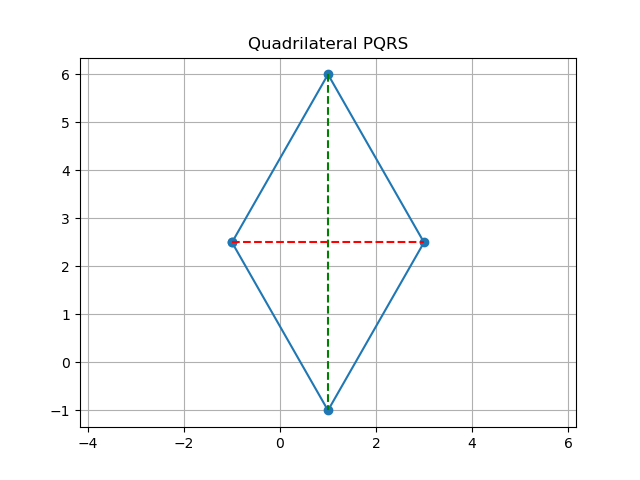
\includegraphics[width=0.5\linewidth]{figs/Figure_1.png}
        \caption{}
        \label{fig:1}
    \end{figure}
\end{center}
    


So,

\begin{center}
\begin{align}
P = \frac{1}{2}(A + B) = \frac{1}{2} \myvec{-1 + (-1) \\ -1 + 6} = \myvec{-1 \\ 2.5}\\
Q = \frac{1}{2}(B + C) = \frac{1}{2} \myvec{-1 + 3 \\ 6 + 6} = \myvec{1 \\ 6}\\
R = \frac{1}{2}(C + D) = \frac{1}{2} \myvec{3 + 3 \\ 6 + 1} = \myvec{3 \\ 3.5}\\
S = \frac{1}{2}(D + A) = \frac{1}{2} \myvec{3 + (-1) \\ 1 + (-1)} = \myvec{1 \\ 0}
\end{align}

Diagonal PR:

$\text{Midpoint}_{PR} = \frac{1}{2}(P + R) = \frac{1}{2} \left( \myvec{-1 \\ 2.5} + \myvec{3 \\ 3.5} \right) = \myvec{1 \\ 3}$

\vspace{0.3cm}

Diagonal QS:

$\text{Midpoint}_{QS} = \frac{1}{2}(Q + S) = \frac{1}{2} \left( \myvec{1 \\ 6} + \myvec{1 \\ 0} \right) = \myvec{1 \\ 3}$

\vspace{1cm}

\textbf{Conclusion}\\
Since O is the midpoint of both diagonals PR and QS, the diagonals of quadrilateral PQRS bisect each other.



\end{document}